% \documentclass[12pt]{article}


%%%%%%%%%%%%%%%%%%%%%%%%%%%%%%%%%%%%%%%%%%%%%%%%%%%%%%%%%%%%%%%%%%%%%%%%%%%
\RequirePackage{etoolbox}
\csdef{input@path}{%
	%{sty/}% cls, sty files
	{img/}% eps files
}%


\documentclass[12pt]{article}

% packages
\usepackage{amsmath}
\usepackage{amssymb}
\usepackage{amsbsy}
\usepackage{amsthm}
\usepackage{mathtools}
\usepackage{mathbbol}
\usepackage{mathrsfs}
\usepackage{bbm} 
\usepackage{graphicx,psfrag,epsf}
\usepackage{enumerate}
\usepackage{natbib}
\usepackage{url} 
\usepackage{float}
\usepackage[skip=5pt]{caption}
\usepackage{subcaption}
\usepackage[normalem]{ulem}
\usepackage{comment}
\usepackage{hhline}
\usepackage{afterpage}
\usepackage{multirow}
\usepackage{adjustbox}
\usepackage{textcomp}
\usepackage{rotating}
\usepackage{tabularx}
\usepackage{xspace}
\usepackage{xr-hyper}
\usepackage[colorlinks,citecolor=blue,urlcolor=blue,filecolor=blue,backref=page]{hyperref}
\usepackage{color,colortbl,soul}
\usepackage[dvipsnames]{xcolor}
\usepackage{blkarray}
\usepackage{tikz}
\usepackage[boxed, vlined]{algorithm2e}
\usepackage[T1]{fontenc}
\usepackage{arydshln}
\usepackage{scalerel,stackengine}
%\usepackage[hmargin=1.0in,vmargin=1.0in]{geometry}

% algorithm options
\SetAlCapSkip{.5em}

% colors
\definecolor{Gray}{gray}{0.9}


\allowdisplaybreaks

% commands
\makeatletter
\renewcommand*\env@matrix[1][*\c@MaxMatrixCols c]{%
	\hskip -\arraycolsep
	\let\@ifnextchar\new@ifnextchar
	\array{#1}}
\makeatother

\newcommand{\iidsim}{\overset{iid}{\sim}} % iid 

\newcommand{\highlight}[1]{%
	\colorbox{yellow!50}{$\displaystyle#1$}}

\DeclarePairedDelimiter\ceil{\lceil}{\rceil}
\DeclarePairedDelimiter\floor{\lfloor}{\rfloor}

\newcommand{\matrow}[2]{{#1}\texttt{[{#2},:]}}

\newcommand{\given}{\,|\,}


\stackMath
\newcommand\reallywidehat[1]{%
	\savestack{\tmpbox}{\stretchto{%
			\scaleto{%
				\scalerel*[\widthof{\ensuremath{#1}}]{\kern-.6pt\bigwedge\kern-.6pt}%
				{\rule[-\textheight/2]{1ex}{\textheight}}%WIDTH-LIMITED BIG WEDGE
			}{\textheight}% 
		}{0.5ex}}%
	\stackon[1pt]{#1}{\tmpbox}%
}

\makeatletter
\newcommand*{\addFileDependency}[1]{% argument=file name and extension
  \typeout{(#1)}
  \@addtofilelist{#1}
  \IfFileExists{#1}{}{\typeout{No file #1.}}
}
\makeatother

\newcommand*{\myexternaldocument}[1]{%
    \externaldocument{#1}%
    \addFileDependency{#1.tex}%
    \addFileDependency{#1.aux}%
}


\def\mathcolor#1#{\@mathcolor{#1}}
\def\@mathcolor#1#2#3{%
	\protect\leavevmode
	\begingroup
	\color#1{#2}#3%
	\endgroup
}

% symbols
\renewcommand{\tilde}[1]{\widetilde{#1}}

%\newcommand{\bm}[1]{\mathbf{#1}}

\newcommand*\rot{\rotatebox{60}}

\usepackage{algorithmicx}
\usepackage{algpseudocode}


\usepackage{tcolorbox}
\newtcolorbox[auto counter]{reviewcommentinside}[1][]{box align=center,
    width=0.9\textwidth,
    colframe = teal,
    colback=teal!10,
    code={\spacingset{0.9}},
    #1}

\newenvironment{reviewercomment}{%
\begin{center}
\begin{reviewcommentinside}\noindent \footnotesize 
}
{\end{reviewcommentinside}
\end{center}}

% draw dag
\usepackage{tikz}
\usetikzlibrary{bayesnet}

\newcommand{\others}{\textrm{---}}
%%%%%%%%%%%%%%%%%%%%%%%%%%%%%%%%%%%%%%%%%%%%%%%%%%%%%%%%%%%%%%%%%%%%%%%%%%%

% DON'T change margins - should be 1 inch all around.
\addtolength{\oddsidemargin}{-.5in}%
\addtolength{\evensidemargin}{-1in}%
\addtolength{\textwidth}{1in}%
\addtolength{\textheight}{1.7in}%
\addtolength{\topmargin}{-1in}%

\begin{document}

\def\spacingset#1{\renewcommand{\baselinestretch}%
{#1}\small\normalsize} \spacingset{1}

\date{}

\newcommand{\footremember}[2]{%
    \footnote{#2}
    \newcounter{#1}
    \setcounter{#1}{\value{footnote}}%
}
\newcommand{\footrecall}[1]{%
    \footnotemark[\value{#1}]%
} 

\newcommand{\bbR}{\mathbb{R}}
\newcommand{\bX}{\boldsymbol{X}}
\newcommand{\bs}{\boldsymbol{s}}
\newcommand{\Ytilde}{\tilde{Y}}

%%%%%%%%%%%%%%%%%%%%%%%%%%%%%%%%%%%%%%%%%%%%%%%%%%%%%%%%%%%%%%%%%%%%%%%%%%%%%%
\newcommand{\mytitle}{My title}  

\title{\bf \mytitle}
\author{Justice Akuoko-Frimpong, Jonathan Ta \and Author Two }

\maketitle


\spacingset{1.9} % DON'T change the spacing. JASA template: 1.9!


\section{Introduction}
\label{sec:intro}
Spatial heterogeneity in environmental processes presents significant challenges for traditional regression modeling approaches. Consider air pollution monitoring across an urban-rural gradient: the relationship between particulate matter (PM2.5) concentrations and predictor variables like traffic density or industrial emissions often varies substantially across space. Global regression models that assume constant coefficients fail to capture these localized relationships, potentially leading to incorrect scientific conclusions and suboptimal policy decisions.
Our work develops a computationally efficient Bayesian implementation of spatially varying coefficient (SVC) models, which address this limitation by allowing regression coefficients to change smoothly over space. Let $s_i \in \bbR^2$ for each $i = 1, \dots, n$ denote spatial locations where we observe response variables $Y(\bs)$ and covariates $\bX(\bs) = (X_1(\bs), \dots, X_p(\bs))^\top$. The SVC model specification:
\begin{align*}
    Y(\bs) = \sum_{j=1}^p X_r(\bs)w_r(\bs) + \epsilon(\bs),
\end{align*}

where $w_r(\bs)$ are spatially varying coefficients modeled as Gaussian processes:

\begin{align*}
    w_r &\sim \text{GP}(0, C(s, s')) \\
    C(s, s') &= \sigma_r^2\exp{(-\phi_r^{-1}\|s-s'\|^2)}
\end{align*}
with $\epsilon(\bs) \sim \text{MVN}(0, \tau^2 I_n)$ representing measurement error.
The key innovations in our implementation include:

\subsection*{Computational Algorithm}
We implement a Markov Chain Monte Carlo (MCMC) algorithm with three key innovations:

\begin{enumerate}
    \item \textbf{Low rank Gaussian Process}: Using knots to reduce the $O(n^3)$ computational complexity of Gaussian process models.
    
    \item \textbf{Adaptive Metropolis-Hastings}: For updating spatial range parameters $\phi_r$ with automatic tuning of proposal distributions:
    \begin{align*}
        \phi_r^{(new)} = \phi_r^{(current)} + \epsilon, \quad \epsilon \sim N(0, \sigma_{adapt}^2)
    \end{align*}
    where $\sigma_{adapt}^2$ adjusts based on acceptance rates during burn-in.
    
    \item \textbf{Efficient linear algebra}: Utilizing Cholesky decompositions for all covariance matrix operations, with pre-computation of constant distance matrices:
\end{enumerate}

\section{Methods}
\label{sec:methods}

\subsection{SVC Model}
\label{sec:model}

Let $s_i \in \bbR^2$ for each $i = 1, \dots, n$ denote a spatial location for which we have collected data, and $\bs = (s_1, \dots, s_n)^\top$ be the vector of all such locations. Then $Y(\bs)$ are univariate dependent variables and $\bX(\bs) = (X_1(\bs), \dots, X_p(\bs))^\top$ are $p \times 1$ vectors of covariates. A linear regression model with spatially varying coefficients assumes $Y(\bs)$ are dependent on $\bX(\bs)$ as follows:
\begin{align*}
    Y(\bs) = \sum_{j=1}^p X_r(\bs)w_r(\bs) + w_0(\bs) + \epsilon(\bs),
\end{align*}
where $w_r(\bs)$ are the regression coefficients corresponding to $X_r(\bs)$, $w_0(\bs)$ are spatial random effects, and $\epsilon(\bs)$ are independently and identically distributed multivariate normal (MVN) measurement errors, i.e.
\begin{align*}
    \epsilon(\bs) \sim \text{MVN}(0, \tau^2 I_n).
\end{align*}
For convenience, we will treat $w_0(\bs)$ as the regression coefficients corresponding to $X_0(\bs) = \mathbf{1}_n$, a vector of length $n$ with every element equal to $1$.

For each $w_r(\bs)$, we assign a Gaussian process (GP) prior with squared exponential covariance, i.e.
\begin{align*}
    w_r &\sim \text{GP}(0, C(s, s')), \text{ where}\\
    C(s, s') &= \sigma_r^2\exp\{\phi_r^{-1}\|s-s'\|^2\}.
\end{align*}
We refer to $C(\cdot, \cdot)$ as the covariance function, which calculates the covariance between two locations $s$ and $s'$. Squared exponential covariance is a commonly used covariance function due to useful properties such as infinite smoothness and gradual decrease in covariance with distance. The parameter $\sigma_r^2$ is the spatial variance and $\phi_r$ is the spatial decay, which indicates how quickly correlation decreases with the squared distance.

We assign inverse-gamma conjugate priors for the variance parameters $\tau^2$ and each $\sigma_r^2$. In addition, each $phi_r$ is assigned a uniform prior. In summary,
\begin{align*}
    & \tau^2 \sim \text{Inv.Gamma}(\alpha_\tau, \beta_\tau),\\
    & \sigma_r^2 \sim \text{Inv.Gamma}(\alpha_r, \beta_r), \text{ and}\\
    & \phi_r \sim \text{Uniform}(l_r, u_r).
\end{align*}

\subsection{MCMC Algorithm}
\label{sec:mcmc}

The primary function in the svc package, svclm, samples from the joint posterior distribution of $w_r(\bs), \phi_r, \sigma_r^2,$ and $\tau^2$, for $r = 0, \dots, p$ using a Gibbs sampler. We will explain how each parameter is sampled at iteration $t+1$.

\subsubsection{Spatial Decay}
\label{sec:spatial_decay}

The parameter $\phi_r^{(t+1)}$ is updated via a random walk Metropolis algorithm. Because $\phi_r^{(t)} \in (l_r, u_r)$, each proposal is calculated as 
\begin{align*}
    \phi_r' &= f^{-1}(f(\phi_r^{(t)}) + U) = l_r + \frac{u_r - l_r}{1 + \exp\left\{\log\left(\frac{u_r - l_r}{\phi_r^{(t)} - l_r} - 1\right) + U\right\}},
\end{align*}
where $U$ is sampled from a normal distribution with mean $0$.

The initial standard deviation for $U$ is specified using the "phi\_proposal\_sd\_start" argument or is $1$ by default. Then the standard deviation is updated at each iteration via a Robust Adaptive Metropolis (RAM) algorithm (Vihola 2012).

\subsubsection{Spatially Varying Coefficients}
\label{sec:svcs}

Let $\Ytilde(\bs) = Y(\bs) - \sum_{j\neq r} X_j(\bs)w_j^{(t)}(\bs)$. Then
\begin{align*}
    \frac{\Ytilde}{X_r}(\bs) | w_r^{(t)}(\bs), \tau^2 \sim \text{MVN} \left(w_r^{(t)}(\bs), \tau^{2(t)} \text{diag}\left( \frac{1}{X_r^2(\bs)} \right)\right) := \text{MVN} \left(\mu, \Sigma\right).
\end{align*}
Then assuming the prior $w_r(\bs) \sim \text{MVN}\left(0, \sigma_r^{2(t)} C\left(\phi_r^{(t)}\right)\right) := \text{MVN}\left(0, \Sigma_0\right)$, we sample $w_r^{(t+1)}(\bs)$ from MVN$(\mu_1, \Sigma_1)$, where
\begin{align*}
    \Sigma_1 &= \left(\Sigma_0^{-1} + \Sigma^{-1}\right) \text{ and }
    \mu_1 = \Sigma_1 \Sigma^{-1} \frac{\Ytilde}{X_r}(s).
\end{align*}

\subsubsection{Spatial Variance}
\label{sec:spatial_variance}

We sample $\sigma_r^{2(t+1)}$ from Inv.Gamma$\left(\alpha_r + \frac{n}{2}, \beta_r + w_r^{(t)}(\bs)^{\top} C\left(\phi_r^{(t)}\right)^{-1} w_r^{(t)}(\bs)\right)$.

\subsubsection{Nugget}
\label{sec:nugget}

We sample $\tau^{2(t+1)}$ from Inv.Gamma$\left(\alpha_t + \frac{n}{2}, \beta_t + \frac{1}{2} \left(Y(\bs) - \sum_{j=0}^p X_r(\bs)w_r^{(t)}(\bs) \right)\right)$.

\section{Data Analysis}
\label{sec:data analysis}
The real world data used in this section is a gridded satellite data with latitude, longitude, temperature, Normalized Difference Vegetation Index (NDVI); which measures vegetation health/greenness, and emissivity which represents a surface's efficiency in emitting thermal radiation. We used temperature as a univariate outcome and used emissivity and NDVI as covariates.
% Figure ref{fig:spatial_patterns} below reveals the spatial  distributions of the variables in the dataset.
% \begin{figure}[h]
% \centering
% 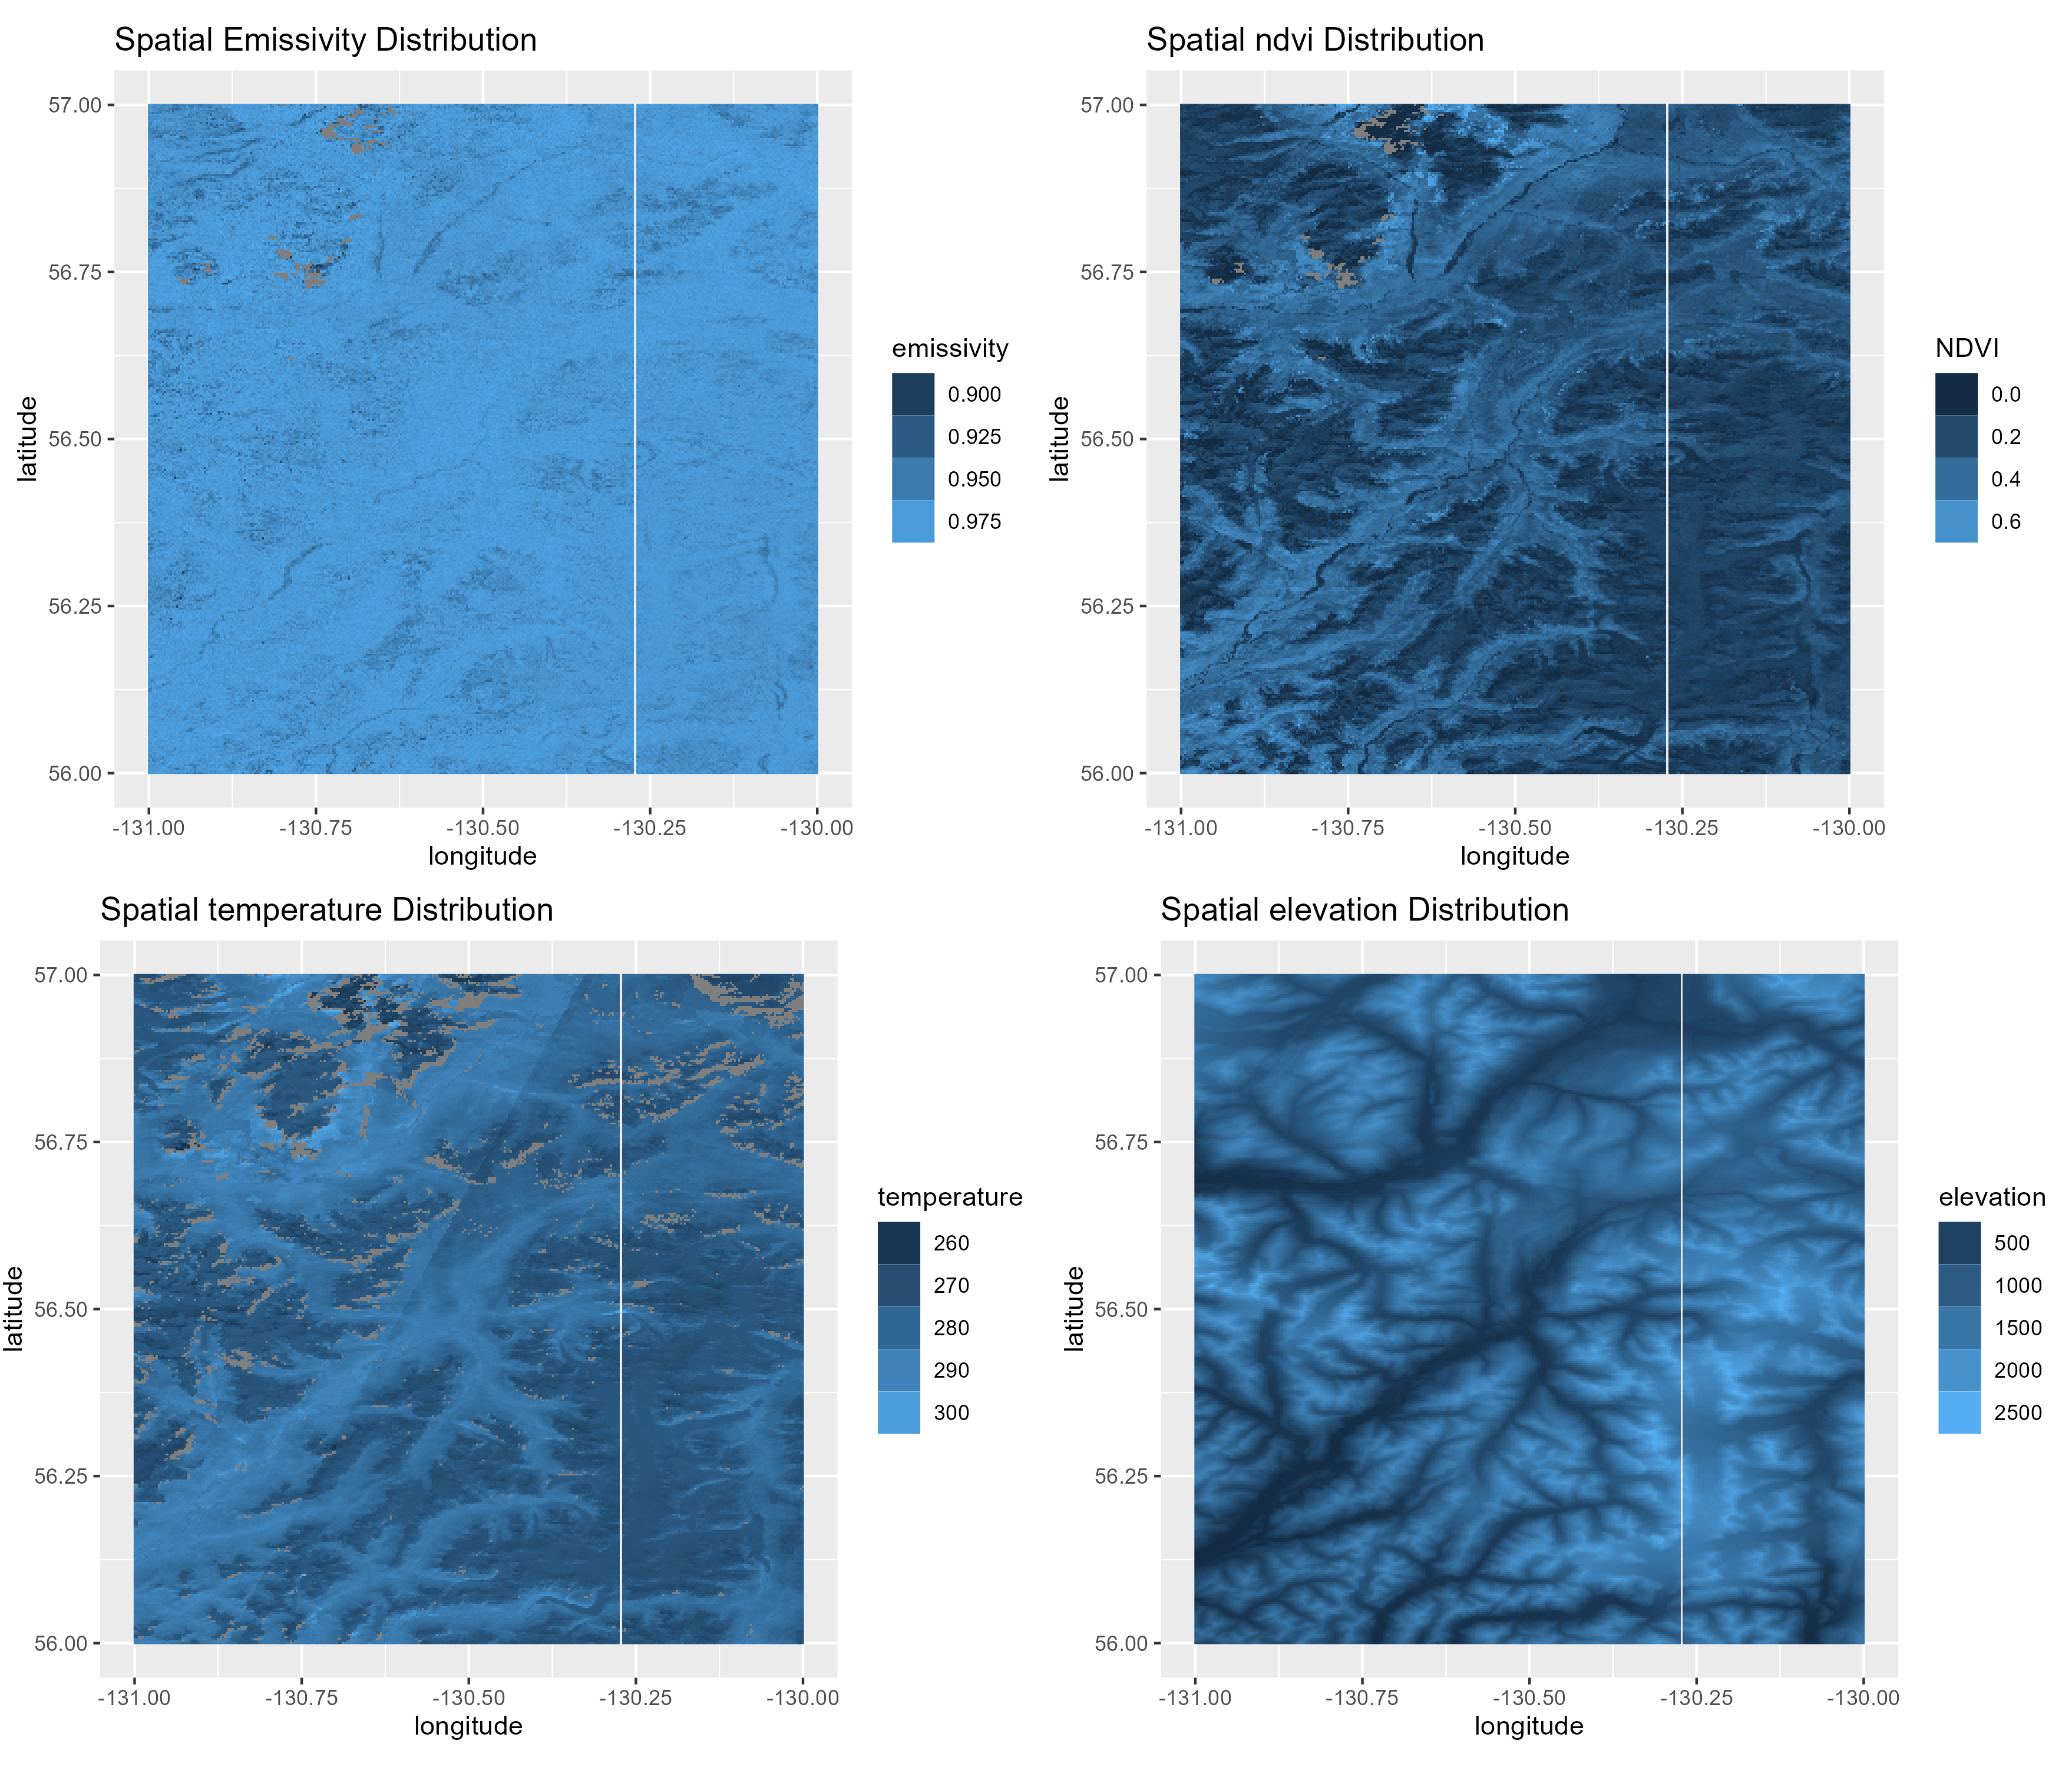
\includegraphics[width=\textwidth]{figures/spatial_horizontal_stack.png}
% \caption{
%   Spatial distributions of emissivity, NDVI, and  land surface temperature in the study area. 
% }
% \label{fig:spatial_patterns}
% \end{figure}
% 
% Emissivity ranges from 0.88 to 0.96. Light blue zones (ε > 0.94) displays dense vegetation/water bodies (high thermal emission efficiency)
% while dark blue clusters (ε ≈ 0.88-0.90) represents urbanized areas. Notice that notice that areas with high NDVI also tend to have higher emissivity which makes sense because vegetation emits efficiently.
% Cooler regions often align with greener (higher NDVI) areas — vegetation can reduce surface temperature through evapotranspiration. \newline
% We computed the empirical semivariograms for the variables in the dataset. 
% \begin{figure}[h]
% \centering
% 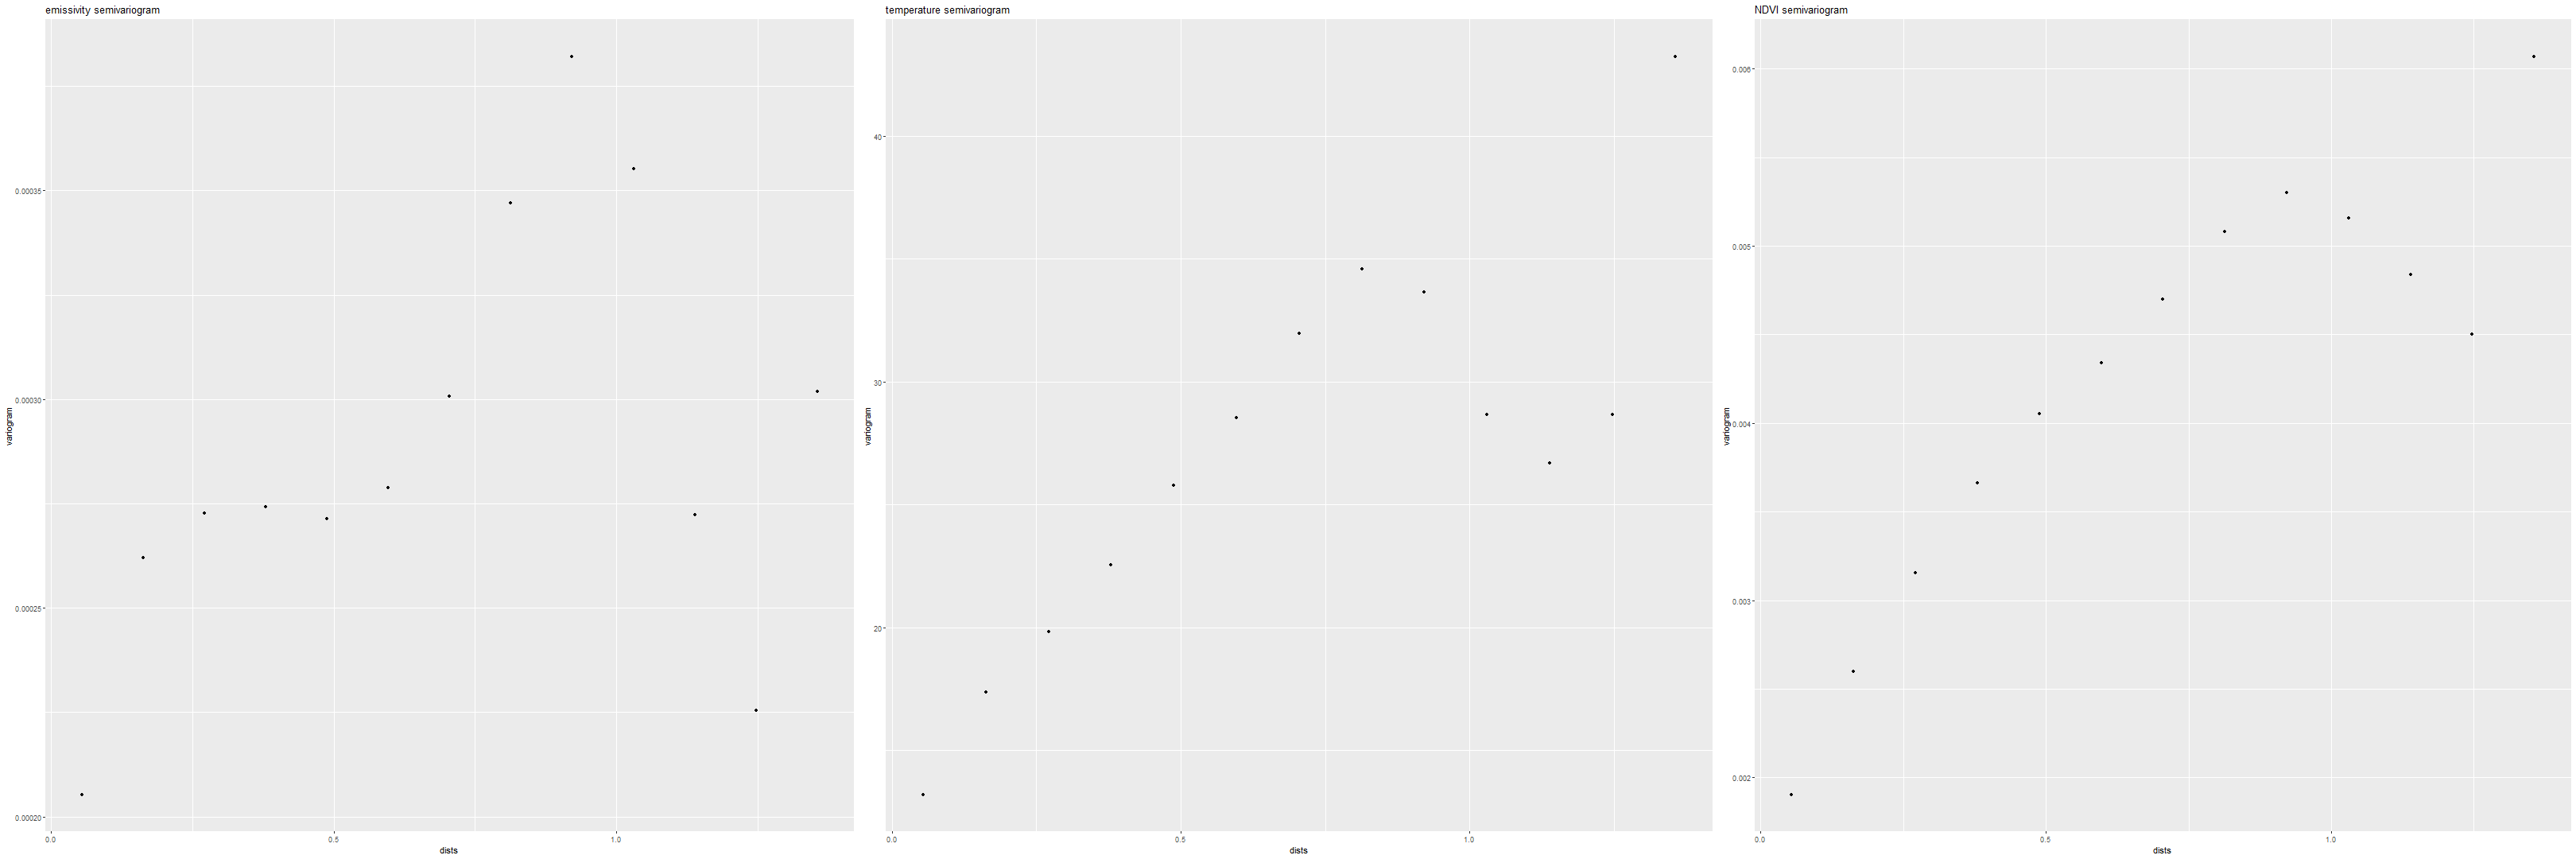
\includegraphics[width=\textwidth]{figures/semivariograms.png}
% \caption{Empirical semivariograms for emissivity, temperature and NDVI}
% \label{fig:semivariograms}
% \end{figure}
The variables showed moderate spatial autocorrelation with low to moderate variance.

\subsection{Model fitting}




\section{Conclusion}
Conclusion


\bibliographystyle{agsm}

\bibliography{bibliography}
\end{document}